% !TEX TS-program = pdfLaTeX+shellescape
% !TEX encoding = UTF-8 Unicode

\documentclass[class=beamer,tikz]{standalone}
\setbeamertemplate{navigation symbols}{} % For delete the navigation symbols
\usefonttheme{professionalfonts}
\usepackage{luatexja}
% \usepackage{pgfplots}
% \pgfplotsset{compat=1.17}

\usepackage{colortbl,array,xcolor}
\usepackage{amsmath,amsfonts}
\usepackage{bm}

\begin{document}
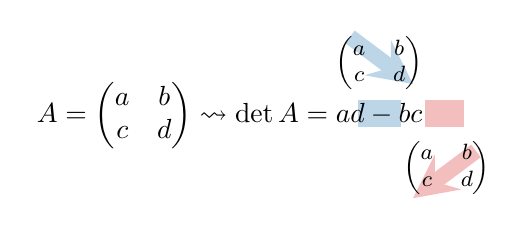
\begin{tikzpicture}
    \definecolor{tab_red}{HTML}{d62728}
    \definecolor{tab_blue}{HTML}{1f77b4}
    \definecolor{tab_green}{HTML}{2ca02c}
    \definecolor{tab_brown}{HTML}{8c564b}
    %\draw[help lines] (0,0) grid (10,6);

    \path[fill=tab_blue!30] (5.20,2.85) rectangle (5.75,3.20);
    \path[fill=tab_red!30] (6.05,2.85) rectangle (6.55,3.20);
    \draw[-stealth, color=tab_blue!30, line width=2.0mm] (5.1,4.0) -- (5.9,3.4);
    \draw[-stealth, color=tab_red!30, line width=2.0mm] (6.7,2.55) -- (5.9,1.95);
    
    % \path[fill=tab_blue!30] (5.05,4.10) -- (5.30,4.10) -- (5.90,3.70) -- (5.90,3.40) -- (5.65,3.40) -- (5.05,3.80) -- cycle;
    % \path[fill=tab_red!30] (6.70,2.65) -- (6.45,2.65) -- (5.95,2.20) -- (5.95,1.90) -- (6.20,1.90) -- (6.70,2.35) -- cycle;
    \node[anchor=west] (matrix) at (1,3.0) {
        $A = \begin{pmatrix} 
            a & b \cr 
            c & d 
        \end{pmatrix} \leadsto \det A = ad-bc$
    };
    \node[anchor=south] (matrix1) at (5.47, 3.20) {
        \footnotesize$\begin{pmatrix} 
            a & b \cr 
            c & d 
        \end{pmatrix}$
    };
    \node[anchor=north] (matrix2) at (6.33, 2.80) {
        \footnotesize$\begin{pmatrix} 
            a & b \cr 
            c & d 
        \end{pmatrix}$
    };
    
    
\end{tikzpicture}
\end{document}